\documentclass{article}
%% Chapter 2 Section 4: Adjoints

\usepackage{amsmath}
\usepackage{palatino}
\usepackage{tikz}

\newcommand{\one}{\mathbf{1}}
\newcommand{\cat}{\mathbf{C}}
\newcommand{\id}{\mathbf{id}}
\newcommand{\pifun}{\mathbf{\Pi}}
\newcommand{\diagfun}{\mathbf{\Delta}}

\begin{document}

\begin{enumerate}
\item [2.4.5]
  \begin{description}
  \item [Unit:]
    Not certain about this, but I think the unit diagram is:
    \begin{center}
      \begin{tikzpicture}
        \node (1) {$\one$};
        \node [right of=1, xshift=1cm] (2) {$\one$};
        \node [below of=2, yshift=-1cm] (3) {$\one$};
        
        \draw[->] (1) -- node [above] {$\iota$} (2);
        \draw[->] (1) -- node[left] {$f$} (3);
        \draw[->] (2) -- node [right] {$T~f^{\#}$} (3);
      \end{tikzpicture}
    \end{center}
    The natural transformation $\iota : \one \rightarrow \one$ is defined by Pierce thus constraining the top two nodes and the functor $T : \cat \rightarrow \one$ is the right adjoint, constraining the bottom node to be $\one$.
    The category $\cat$ is only involved with the function $f^{\#}$.
    It acts the single $\cat$-object obtained by lifting the unique object of $\one$ into $\cat$.

    Not sure how to identify the initial object or the existence of unique arrows.
  %% \item[]
  %% \item [Co-unit:]
  %%   I \emph{think} the counit diagram is:
  %%   \begin{center}
  %%     \begin{tikzpicture}
  %%       \node (1) {$\cat$};
  %%       \node [below of=1, yshift=-1cm] (2) {$\cat$};
  %%       \node [right of=1, xshift=1cm] (3) {$\cat$};
  %%       \draw[->] (2) -- node [left] {$F~g^*$} (1);
  %%       \draw[->] (2) -- node[above] {$\varepsilon$} (3);
  %%       \draw[->] (1) -- node [right] {$g$} (3);
  %%     \end{tikzpicture}
  %%   \end{center}
  \end{description}
\item[]
\item[2.4.7]
  We have a category $\cat$ with products, a product functor $\pifun : \cat \rightarrow \cat \times \cat$ and a diagonal functor $\diagfun : \cat \times \cat \rightarrow \cat$.
  The diagram for the unit is:
  \begin{center}
    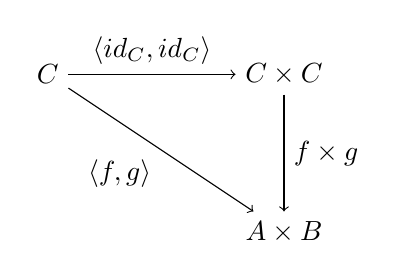
\begin{tikzpicture}
      \node (1) {$C$};
      \node[right of=1,xshift=2cm] (2) {$C \times C$};
      \node[below of=2,yshift=-1cm] (3) {$A \times B$};

      \draw[->] (1) -- node[above] {$\langle id_C, id_C \rangle$} (2);
      \draw[->] (1) -- node[below left] {$\langle f , g \rangle$} (3);
      \draw[->] (2) -- node[right] {$f \times g$} (3);
    \end{tikzpicture}
  \end{center}

  And the diagram for the counit is:
  \begin{center}
    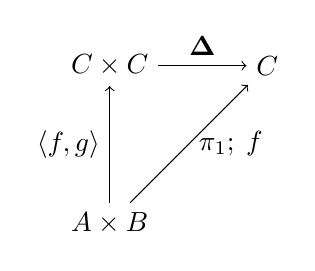
\begin{tikzpicture}
      \node (1) {$C \times C$};
      \node [below of=1,yshift=-1cm] (2) {$A \times B$};
      \node [right of=1,xshift=1cm] (3) {$C$};
      
      \draw[->] (2) -- node[left] {$\langle f , g \rangle$} (1);
      \draw[->] (2) -- node[right] {$\pi_1;~f$} (3);
      \draw[->] (1) -- node[above] {$\diagfun$} (3);
    \end{tikzpicture}
  \end{center}
  To show that $A \times B$ satisfies the definition of a product, we need to find projection arrows $\pi_1 : A \times B \rightarrow A$ and $\pi_2 : A \times B \rightarrow B$ and guarantee that for any object $C$ with arrows $f : C \rightarrow A$ and $g : C \rightarrow B$ we have a unique arrow $\langle f, g \rangle : C \rightarrow A \times B$.
  The counit diagram provides our projection arrows and the uniquely determined function $f \times g \circ \langle \id_C \times \id_C \rangle$ of the unit diagram gives the map from $C$ to $A \times B$.
\end{enumerate}
\end{document}
